
\chapter{System Concept and Methodology}
\label{CH_3_System Concept and Methodology}

\section{Problem Definition and Objectives}
\label{Problem-Definition-and-Objectives}

The state of the art has shown clearly that industrial robots are widely used for the press brake sheet metal bending, primarily through manual programming or predefined programming methods. These methods perform well in structured scenarios with fixed part position, geometries, and bending sequences. However, as product variants increase, the adoption of such robot programming approaches requires manual reprogramming and time consuming.
\par In press brake bending, after each bending operation, the shape of the sheet metal changes. Each geometric change affects robot reachability, gripping feasibility and grip point calculations, motion trajectories. Consequently, handling and regripping should be planned carefully. Previous research shows that managing this constraint is one of the most time-consuming and complex aspects of robotic bending processes particularly when handled manually. 
\par From a methodological perspective, the limitations of this robot programming approaches related to their low-level nature. programmers must define the robot paths, position of tools and individual waypoints. This makes the programming, tightly coupled to a specific robot, grip positions or tool setups and making the reorientation or regripping strategies difficult to adapt. Robotic literature clearly indicates that such low-level programming does not scale well as system complexity increases and flexibility requirements grow \cite{Siciliano2016Robotics}.
This observation motivated research into the higher-level representation, where motion execution and decision making integrated with a unified framework. These methods aim to simplify handling constraints and promote reusable robot programs. While these strategies have been implemented in other robotic applications, they have not yet been implemented in robotic press brake sheet metal bending, particularly when the position and geometry changes must be explicitly considered.
\par Based on these observation , the central problem addressed in this thesis can be defined as follow: There is a lack of a systematic approach for automatic generation of robot programs for press brake sheet metal bending that explicitly accounts for changing workpiece positions and geometry , handling feasibility and regripping requirements while minimizing the manual programming .
\par The primary objective of this thesis is to develop a conceptual and methodological framework for the automatic generation of the robot program that integrates bending, handling and regripping operations in one workflow. This proposed method aims to reduce manual programming effort and improve adaptability to different part geometries. To achieve this objective ,the work focuses on integrating bending sequences , handling actions , opposite side bending and regripping operation and which are validated and verified in simulation environment compatible with industrial robot environment .The scope of the thesis is limited to virtual environment and conceptual evaluation.
%%%%%%%%%%%%%%%%%%%%%%%%%%%%%

\section{Requirement Definition and Management}
\label{Requirement-Definition-and-Management}

To ensure a systematic and verifiable development of the proposed automatic robot program generation approach, the system design is guided by explicitly defined requirements. These requirements turn the research gap and problem formulation into engineering objectives that can later be verified and validated.
The requirement that are explained in this chapter are directly derived from the limitations identified in the state of art and from the objectives formulated in \ref{Problem-Definition-and-Objectives}. Rather than describing implementation details , the requirement specify  what the system must achieve under which condition it must operate .This separation ensures that design decision  remain traceable and that verification activities can be performed objectively.
The requirement are classified into functional and non-functional requirements .Functional requirements describe the expected system behavior and capabilities , while nonfunctional requirements define the quality attributes such  as usability , robustness and safety .In addition , system constraints and assumptions are explicitly stated to scope of the work and to define the operational boundaries of the proposed solution
To support systematic verification, each requirement is formulated to Specific measurable Achievable Relevant Timebound (SMART) principle. Furthermore, each requirement is linked to system components and verifications steps. This traceability ensures that all requirements can be checked later and that the development process remains transparent and consistent.
   
\subsection{Functional Requirements}
\label{functional-Requirement}

Functional requirements specify the capabilities that the system provides in order to address the problem of automatic robot program generation for press brake sheet metal bending. These requirements define the expected system behavior from the task execution, operator interaction, trajectory generation and recovery mechanism.
At a high level, the system shall enable the automatic generation of robot programs for multi-step sheet metal bending process without requiring manual t programming. The system shall support the execution of bending sequences that involve changes in workspace geometry, orientation, handling and regripping strategies.
\par A central functional aspects of the system is the consideration of work piece geometry evolution during bending process .Since the shape , position , orientation of the sheet metal changes after each bending operations , the system shall be feasible to handle the current geometric state and position of the workpiece when generating subsequent actions for the next task. This requirement is essential to ensure feasibility with respect to robot reachability and tool operations throughout bending sequence.
Furthermore , the system shall support bending operations that requires for different sides of the work piece .Opposite side bending introduces additional constraint on tool orientation and  robot configuration , which cannot always be resolved with a fixed handling strategy and time consuming .The system program therefore capable of adapting this strategy , including workpiece orientation and grip configuration, to enable such operation while maintaining feasibility
\par To structure the functional requirements, they are grouped into categories.
\paragraph{Operator Interaction Requirements:} 
The system shall allow limited operator interaction for configuration of robot and process selection while minimizing the manual intervention during the execution. Before execution, the operator shall be able to specify the required process output, such side for bending or cad model for bending. During execution, the robot operation shall provide clear feedback or warning message when the given output conditions are unsafe for the process. The role of operator shall be restricted to configuration, while the program generation logic shall be handled automatically by the system.
\paragraph{Data Handling Requirements:}
The system should automatically use the operator input data and process the program that need to processed for the required output in a consistent and reliable manner .This includes Handling geometries , grip position calculation, tracked poses , configuration parameters and intermediate state information generated during the time of execution. Data shall be used consistently across different stage of the program generation process to ensure that decisions regarding the handling and orientation and regripping are based on the current system state.
\paragraph{Motion Execution Requirements:}
The system shall generate feasible robot waypoints for all handling and bending related operations. This includes generation of approach waypoints, placement motions and the execution of orientation changes of the work piece and tool. Trajectory plans should be calculated prior to execution to prevent unreachable target poses.
In addition, the system shall determine and apply appropriate grip positions on the workpiece to support handling and picking from different bending configurations. For opposite side bending operations, the system shall identify the grip position and waypoints such that required tool alignment can be achieved without violating the kinematical limits. Grip selection shall be treated as an integral part of the program generation process rather than manual integrated adjustments.
\paragraph{Error Handling and Regripping Requirements:}
The system shall be capable of detecting infeasible target poses or unsafe execution conditions before execution. When such conditions are detected, the system shall initiate a warning message to the user, trigger appropriate recovery actions instead of continuing execution. Recovery actions may include regripping or repositioning the workpiece to restore reachability.
Regripping operation shall be supported as functional capability of the system .The system shall be able to integrate regripping sequence into generated robot program when direct trajectories to the target are unreachable or unsafe .If a critical error cannot be resolved through recovery actions , the system shall terminate execution in controlled regripping or repositioning manner to prevent unsafe robot behavior.
\begin{sidewaystable}[p]
\centering
\caption{Functional Requirements for Automatic Robot Program Generation}
\label{tab:functional_requirements}

\renewcommand{\arraystretch}{2.0}

\begin{tabular}{p{2cm} p{9cm} p{9cm} p{4cm}}
\toprule
\textbf{ID} &
\textbf{Functional Requirement (SMART)} &
\textbf{Acceptance Criteria} &
\textbf{Verification Method} \\
\midrule

FR-01 &
The system shall detect unreachable target poses before robot motion execution. &
The robot shall not execute motion to unreachable poses and shall provide an error message. &
Simulation Based \\

FR-02 &
The system shall allow operator-side selection prior to program execution. &
The selected bend side shall be applied correctly to the generated robot program. &
Simulation Based \\

FR-03 &
The system shall execute a regripping sequence when a target pose is unreachable within the current bend side. &
Regripping shall be performed successfully and execution shall continue without interruption. &
Simulation Based \\

FR-04 &
The system shall handle workpiece orientation changes during program execution. &
Orientation changes shall be applied correctly without violating kinematic limits. &
Simulation Based \\

FR-05 &
The system shall support opposite-side bending operations when required. &
The system shall correctly execute opposite-side bending operations. &
Simulation Based \\

FR-06 &
The system shall determine and apply suitable grip positions for each workpiece state. &
Grip positions shall be determined and applied correctly for each workpiece state. &
Simulation Based \\

FR-07 &
The system shall terminate execution when an unsafe operation is detected. &
The robot shall terminate execution and display an error message. &
Simulation Based \\

\bottomrule
\end{tabular}
\end{sidewaystable}


\subsection{Non-functional Requirements}
\label{non-functional-requirements}

NFR defines the quality attributes and operation characteristics that elaborates how well the system performs its functions. While the functional requirements specify the system capabilities, non-functional requirements describe constraints related to usability, maintainability, robustness and safety. These aspects are important for automated robotic systems, where corrected system behavior alone is not sufficient if the system is difficult to use, fails under complex variations or behaves unsafely during execution.
The NFR of the system are derived from the operational context of press brake sheet metal bending, where industrial robot operates in close proximity to tooling, workpieces and cell boundaries. The system is intended to support flexible manufacturing scenarios with minimal operator programming while maintaining the user conditions and safe behavior. To ensure clarity, the NFRs are grouped into the following categories.
\paragraph{Usability Requirements:}
The system should be designed such that the user can operate the system easily by minimizing the operator interaction during normal operation. 	Configuration steps required prior to execution shall be limited to essential parameters and shall be presented in a clear and understandable manner. The system should give meaningful feedback to operator, including warning information and error messages when unreachable waypoints or unsafe condition are detected. These messages shall support the operator in understanding the cause of an issue without requiring expert knowledge of robot programming.
\paragraph{Maintainability Requirements:}
The system shall support maintainability by enabling configuration changes without requiring modifications to the source code. Process parameters, handling strategies and system setting shall be adjustable through configuration mechanisms that are separated from the core program logic. In addition, the system should provide sufficient logging or terminal output to support debugging, monitoring and future extensions. These measures are intended to facilitate adaptation of the system to new workpiece, process variations, with minimal programming effort.
\paragraph{Robustness Requirements:}
The system shall exhibit robust behavior under repeated execution cycles. Small variations in workpiece, orientation or exceptions timing or path shall not lead to system failure or unsafe behavior. The system shall handle such behavior deviation in controlled manner, ensuring smooth operations whenever feasible or triggering appropriate recovery actions when required. Robustness is particularly important in flexible manufacturing environments where idealized conditions cannot be assumed.
\paragraph{Safety Requirements:}
The system should always ensure safe operations by validating generated robot motion trajectories, informing the user about unsafe conditions and enforcing defined safety constraints and forbidden zones to prevent unreachable or unsafe poses during program execution. In the events of critical errors or unsafe conditions that cannot be resolved through recovery actions, the system shall terminate execution in a controlled manner. 
\begin{table}[htbp]
\centering

\setlength{\tabcolsep}{3pt}
\renewcommand{\arraystretch}{1.0}
\hyphenpenalty=500
\exhyphenpenalty=500

\begin{tabularx}{\textwidth}{
L{1.3cm}
L{5.8cm}
L{4.4cm}
L{3.1cm}
}

\hline
\textbf{ID} &
\textbf{Non-Functional Requirement} &
\textbf{Observable Acceptance Criteria} &
\textbf{Verification Method} \\
\hline

NFR-01 &
Operator interaction during normal automated generation shall be limited to configuration or input selection and execution confirmation. &
The automated workflow comparison shall require no manual waypoint teaching, function-block sequencing, or manual reprogramming before simulated execution. &
Manual-versus-automated workflow validation \\

\hline

NFR-02 &
Workpiece geometry, process settings, and safety parameters shall be configurable without source-code modification. &
Geometry-change and position-change scenarios shall be handled through configuration or operator input updates without rebuilding or modifying source code. &
Geometry and position variation validation \\

\hline

NFR-03 &
Unsafe or infeasible conditions shall produce clear warning or error feedback before continuation. &
Detected unsafe or infeasible conditions shall generate warning or error feedback and shall require operator acknowledgement, replanning, or controlled termination before continuation. &
Failure-prone and warning-behaviour validation \\

\hline

NFR-04 &
The system shall use a deterministic execution sequence for a given configuration. &
Repeated automated runs under the same scenario definition shall produce consistent completion, failure, or controlled-stop classifications. &
Repeated automated scenario validation \\

\hline

NFR-05 &
Fixture pose deviations shall be checked against defined positional and angular tolerance limits before execution. &
Position deviation above 5~mm or angular deviation above 0{,}10~rad shall trigger a fixture warning and controlled operator decision before execution. &
Fixture perturbation and constrained-placement validation \\

\hline
\end{tabularx}

\caption{Non-Functional Requirements -- NFR-01 to NFR-05 with acceptance criteria and verification methods.}
\label{tab:non-functional-requirements}
\end{table}


\subsection{System Constraints and Assumptions}
\label{System-Constraints-and-Assumptions}

In addition to functional and non-functional requirements, the development of the proposed automatic robot program generation system is subject to a defined sets of constraints and assumptions. These Constraints delimit the scope of the thesis and clarify the operational boundaries within which the system is designed to function. Explicitly stating these limitations ensures transparency and prevents misinterpretation of the intended system capabilities.
The proposed approach is developed for a predefined robotic press brake cell configuration. The mechanical layout of the robot, press brake, tooling and auxiliary components is assumed to remain fixed throughout the system operations. Changes to physical robotic position and tool geometry, and non-collision movement planning are out of scope of this work.
The system assumes the availability of accurate geometrical models of the robot, workpiece, press brake, and related components within the virtual environments. The correctness of reachability analysis and motion feasibility check depends on the validaty of these models. Model inaccuracies, calibration errors or unmodeled physical effects are not explicitly compensated within the proposed framework.
Explicitly defining these limitations ensures transparency and prevents over interpretation of the system capabilities.
The constraints are grouped into geometric, process related, cell layout, handling and safety limitations.
\paragraph{Sheet geometry Constraints : }
The system is designed for rectangular sheet metal workpiece only. All geometric reasoning, grip position calculations and edge distance check assumes a rectangular shape with four orthogonal edges. Nonrectangular geometries, polygonal shapes or free form contours are not supported.
The sheet geometry is parameterized by its length, width thickness and mass. Optional circular holes may be defined using radial parameters. However, only circular holes are supported, irregular polygonal cuts are not considered. All hole’s related checks are performed using radial distance evaluation.
Furthermore, only a single global wall height parameter is considered during the handling. Per edge height customization is not supported.
\paragraph{Bend and process constraints:} 
The bending process is restricted to 90 degrees of bend angles. Variable user defined bend angles are not supported. The bending logic assumes one bend per edge and each edge can be associated with at most one bending operation.
A maximum of four bends per side is supported. For opposite side operation, the number of bends is similarly limited to four. The program logic prevents the duplicate bend assignments and multiple bend assignments on the same edge. This ensures a consistent one bend per edge configuration and simplifies the geometric reasoning required for the automatic program generation.
\paragraph{Robot and cell layout constraints:} 
The robotic cell configuration is assumed to be fixed. The robot base, press brake, fixtures and auxiliary components are defined relative to a constant world coordinate frame. Relocation or reconfiguration of these elements invalidates the area logic, reachability assumptions and orientation constraints. In this case, system requires manual updates of configuration values for adaptation.
Tool configuration is also assumed to be fixed. The system operates with a predefined TCP (tool center point) and attachment frame (Flange) Changes tool geometry, TCP definition or IO wiring require configuration updates and may necessitate software adaptation.
Vacuum gripping is controlled via single digital output. Alternative control schemes are not considered.
\paragraph{Gripping constraints:} 
The system is designed exclusively for vacuum based gripping. Grip feasibility checks are based on physical considerations including pressure difference friction and rated shear force. The holding capability of a vacuum gripper depends primarily on the achievable pressure difference between suction cup and the ambient atmosphere, the effective contact area and the frictional interaction between workpieces surfaces and the suction elements.\cite{VacuumGripperModeling}.
Mechanical magnetic or finger-based grippers are not supported within the current framework.
\paragraph{Safety and warning system constraints:} 
The safety and warning logic monitors only a predefined ser of fixtures and reference objects within the cells. Full collision detection, dynamic safety trajectory planning and advanced real time safety validation are not implemented. Safety evaluation is limited to predefined geometric checks and rule-based constraints within virtual environment.
Object tracking and naming assumptions -The systems rely on predefined object identifiers within the virtual environment. Specific object names are expected as key to finding to process or finding the objects. Renaming or removing these objects disrupts the workflow logic and may lead to execution failure. Therefore, renaming objects requires manual updates in the program configuration.

\subsection {Software Platform and Tool requirement}
\label{Software Platform and Tool requirement}
Instead of coming from the functional analysis, the development context imposes three additional requirements. The industrial partner environment and the hardware available within the thesis scope determine the choice of execution platform, the communication interface that allows the planning system to reach the robot runtime, and the physical tool geometry from which all motion targets are computed. As a result, these limitations are formalized as SR-01, SR-02, and SR-03 software and tool platform requirements.
\subsubsection{SR-01 Drag And Bot runtime Platform}
The drag and bot software platform, developed by drag and bot GMBH. The drag and bot runtime will receive and carry out all robot motion commands, service calls, and object management operations produced by the planning modules; this work does not support any other execution environment.
Two main requirements of this thesis serve as the foundation for choosing drag and bot as the execution environment. First, as mentioned in Section \ref{Problem-Definition-and-Objectives}, the work is limited to a virtual environment, and drag and bot offers an integrated simulation runtime that enables thorough validation of robot programs without requiring access to actual robot hardware \cite{dragandbot_anyrobot_2025}. Second, the platform allows the planning system to remain robot-independent at the software level by exposing a uniform application programming interface that abstracts manufacturer-specific robot controller syntax. By executing within the drag and bot virtual environment, the object tracking subsystem, the digital IO interface, and the object attach/detach services all operate under conditions representative of the target press brake cell, ensuring that simulation-based verification as specified for FR-01 through FR-07 is meaningful and reproducible.
The suitability of runtime abstraction layers for controller-independent robot program generation is established in the modular robotic automation literature\cite{Thramboulidis2013MDE}. The drag and bot platform documentation confirms the availability of the virtual simulation environment, the AnyRobot Interface, and the RosBridge communication server on which the system depends. All planning modules developed are implemented exclusively against this API, and all validation test cases are executed within this environment.
\paragraph{ Acceptance Criteria} — SR-01: the planning system shall establish a stable authenticated connection to the drag and bot runtime within 5 seconds of launch; all motion, service, and IO commands shall be dispatched and acknowledged without error during the simulation
\subsubsection {SR-02 Anybot Interface as Exclusive Communication layer.}
The AnyRobot Interface, provided by drag and bot GmbH as part of the drag and bot software stack, shall constitute the sole communication channel between the planning system and the drag and bot runtime \cite{dragandbot_anyrobot_2025}. All robot motion commands: digital IO operations, object manager service calls, and operator requests shall be transmitted exclusively through this interface; direct controller-level communication or any alternative channel is outside the scope of this work.
Because it combines all robot functions into a single WebSocket channel based on the RosBridge v2 protocol, such as LIN and PTP motion commands, vacuum gripper IO, kinematic object attachment, and modal operator dialogs, the AnyRobot Interface is widely used. Without a locally installed ROS environment, messages are sent as JSON-formatted objects that can be created and sent in Python. This architecture directly addresses the NFR-02 maintainability requirement by eliminating the need for a robot-manufacturer-specific post-processor and enabling the planning system to target a different robot model with just a configuration update. Connection security is enforced through a SHA-512-based rosauth authentication handshake at session establishment, ensuring that only the authorized planning client can issue commands to the runtime - a design decision that supports the safety and robustness requirements NFR-03 and NFR-05.
\paragraph{ Acceptance Criteria} — SR-02: all planning-to-runtime communication shall occur exclusively over the AnyRobot WebSocket channel; an authenticated connection shall be established before any command is dispatched; LIN motion, digital IO, object manager commands shall each be successfully executed and acknowledged during the simulation
\subsubsection{SR-03 Tool Centre point.}
The tool center point (TCP) applied to all robot motion targets throughout the planning system shall be defined by the tool configuration registered in drag and bot. The TCP pose relative to the robot flange, expressed in the EULER\_INTRINSIC\_ZYX convention \cite{wiki:euler_angles}, is x = 0.000 m, y = 0.034 m, z = 0.194 m, Rz = −90.0°, Ry = −75.0°, Rx = 0.0°. These values define the geometric offset from the robot flange frame to the contact surface center of the vacuum suction cup mounted on the end-effect.
The tool center point in the world coordinate frame is where all motion targets generated by the planning system are expressed, including pickup poses, pre-bend approach poses, regrip placement poses, and post-bend unload poses. The inverse of the flange-to-TCP transform is used to derive the corresponding flange pose from the TCP target, which is then executed by the robot controller \cite{craig2005robotics}. A positioning error at the workpiece contact surface results from any mismatch between the declared TCP offset and the actual gripper geometry. Such an error would jeopardize the viability of the grip and increase the risk of workpiece slippage during handling in the context of vacuum gripping, where holding force depends on the achievable pressure differential and the effective contact area \cite{VacuumGripperModeling}.
By defining the TCP as a formal, traceable requirement instead of an implicit code constant, design transparency is maintained and future tool replacements are reflected as intentional requirement changes. 
As seen in fig \ref{fig:tcp} , the TCP pose values are registered in the drag and bot tool management system as project\_3\_tcp and are obtained from the physical geometry of the suction gripper assembly installed on the robot within the press brake cell. In accordance with the configuration-driven design required by NFR-02, these values are loaded from the input configuration file at runtime.
\paragraph{ Acceptance Criteria} - SR-03: all motion targets generated during simulation test execution shall produce flange poses consistent with the declared project\_3\_tcp offset; the TCP identifier and pose values shall be loaded exclusively from the YAML configuration file; a change to the TCP pose in the configuration file shall propagate correctly to all generated motion targets without requiring source code modification.
\begin{figure}[htbp]
    \centering
    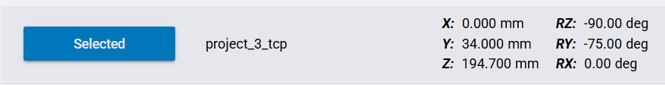
\includegraphics[width=0.7\textwidth]{figures/tcp.png}
    \caption{Tool Center Point parameters in Drag\&Bot.}
    \label{fig:tcp}
\end{figure}

\subsection{System Traceability}
\label{System Traceability}

Requirements Traceability is a fundamental principle in systematic engineering development, ensuring that all defined requirements are consistently reflected in the system design, implementation and validation stages. In the context of the proposed automatic robot program generation system, traceability guarantees that the transition from conceptual objectives to executable functionality remains transparent, structured and verifiable.
Each requirement is defined in section \ref{functional-Requirement} (functional requirement) and Section \ref{non-functional-requirements}(Nonfunctional requirements) is assigned to a unique identifier (e.g. FR-01, NFR -019:) .These identifiers serve as persistent reference throughout the entire development lifecycle. The identifiers are used consistently in the following aspects:
\begin{itemize}
    \item Every requirement is implemented within a specific module.
    \item Every requirement is verified through a defined test scenario.
    \item No requirement remains unnoticed.
    \item No implementation functionality exists without requirement justification.
\end{itemize}
\paragraph{Forward traceability:} confirms that every requirement is realized in a specific system components or logic module.
\paragraph{Backward traceability:} confirms that every implemented functionality can be tracked back to an explicitly defined requirement.\\
By mapping each requirement to a corresponding implementation module and validation scenario , the development process become auditable and reproducible, which is particularly important in systems involving automated decision making , such as traceability evaluation , regripping logic , and opposite side handling .In addition tractability improves  maintainability and future extensibility, such as adapting to a new gripper type or extending bend angle support . This structure allows systematic impact analysis. Affected requirements and modules can be identified quickly, thereby reducing development risk.
\begin{table}[htbp]
\centering
\caption{Requirement Traceability Matrix --- all fifteen requirements (FR-01 to FR-07, NFR-01 to NFR-05, SR-01 to SR-03) mapped to implementation modules and verification scenarios}
\label{tab:req_traceability_matrix}

\setlength{\tabcolsep}{4pt}
\renewcommand{\arraystretch}{1.05}
\scriptsize
\hyphenpenalty=10000
\exhyphenpenalty=10000

\begin{tabularx}{\textwidth}{
L{1.4cm}
L{4.2cm}
L{5.2cm}
L{3.2cm}
}
\toprule
\textbf{Req.\ ID} &
\textbf{Requirement Description} &
\textbf{Implemented In} &
\textbf{Verified In} \\
\midrule

FR-01 &
Detect unreachable target poses before execution. &
Reachability checking and admissibility validation logic &
Simulation test case TC-01 \\

FR-02 &
Allow operator-side selection of bending configuration before execution. &
Operator dialog and configuration collection logic &
Execution test case TC-02 \\

FR-03 &
Execute regripping sequence when a target pose is unreachable. &
Automatic regrip cycle logic with I/O and attach/detach control &
Regrip validation test case TC-03 \\

FR-04 &
Handle workpiece orientation changes during program execution. &
Orientation conversion, rotation normalisation, and strategy selection logic &
Orientation validation test case TC-04 \\

FR-05 &
Support opposite-side bending operations when required. &
Opposite-side bending workflow with sheet-flip and regrip completion logic &
Opposite-side validation test case TC-05 \\

FR-06 &
Determine and apply suitable grip positions for each workpiece state. &
Grip planning logic with edge-clearance, spacing, and vacuum-force feasibility checks &
Grip validation test case TC-06 \\

FR-07 &
Terminate execution when an unsafe operation is detected. &
Safety warning and pre-execution deviation checking logic with operator confirmation dialog &
Safety validation test case TC-07 \\

NFR-01 &
Ensure minimal operator interaction during normal execution. &
Operator interaction limited to bend-side selection and execution confirmation &
Usability validation \\

NFR-02 &
Allow process parameter changes without source code modification. &
Configuration reader and YAML-based single-source process configuration &
Configuration validation test \\

NFR-03 &
Provide clear warning and error messages for unsafe conditions. &
Warning generation and modal operator notification logic &
Warning message validation \\

NFR-04 &
Ensure robustness under repeated execution cycles. &
Deterministic execution loop with automatic waypoint generation and path logging &
Repeated run validation test \\

NFR-05 &
Tolerate moderate pose deviations within defined tolerance limits. &
Configurable pose-deviation threshold and perturbation handling logic &
Perturbation validation test \\

SR-01 &
drag\&bot GmbH runtime platform shall be the exclusive robot execution environment. &
Runtime client connection logic for communication with the configured drag\&bot host and port &
Platform integration check: runtime connection and command dispatch verified \\

SR-02 &
AirRobot Interface shall be the exclusive software communication layer between planning system and robot runtime. &
Authenticated WebSocket communication layer with JSON command exchange &
Interface integration check: authenticated connection and JSON command round-trip verified \\

SR-03 &
TCP shall be configured as project\_3\_tcp: $x=0.000$ m, $y=0.034$ m, $z=0.194$ m, $R_x=-90.0^\circ$, $R_y=-50.0^\circ$, $R_z=0.0^\circ$. &
Default TCP pose definition applied in all flange-to-TCP transformations &
TCP configuration check: flange pose computed correctly for reference target poses \\

\bottomrule
\end{tabularx}

\end{table}

%%%%%%%%%%%%%%%%%%%%%%%%%%%%%%%%%%
